% !TEX root = ../paper.tex
\label{sec:patternmixtureencodings}
Thus far we have defined the problem of log compression, treating the query log as a multivariate distribution $p(Q)$ where patterns capture positive frequencies of feature (co-)occurrence.
However in cases like logs of \textit{mixed} workloads, there are also many cases of anti-correlation between features.
For example, consider a log that includes queries drawn from a mixture of two workloads with disjoint feature sets.
Pattern-based summaries can not convey such anti-correlations easily.
As a result, patterns including features from both workloads never actually co-occur in the log, but a pattern-based summary of the log will suggest otherwise.
Such false positives are especially problematic for use-cases of \systemname involving outlier detection (e.g., \cite{DBLP:conf/trustcom/KulUC18}).
Even in other settings, capturing correlations reduces data dimensionality and improves both runtime and effectiveness of state-of-the-art pattern mining algorithms (See Section~\ref{sec:evaluatingalternativeapplicationsexperiments}).
%In addition, by detecting and separating groups of anti-correlated features, one can partition the data accordingly and reduce data dimensionality for each partition.
%, which causes pattern based encoding schemes to break down in terms of computation efficiency.% (shown in Section~\ref{sec:refiningnaivemixtureencodings}). 

In this section, we propose a generalization of pattern encodings where the log is modeled not as a single probability distribution, but rather as a mixture of several simpler distributions.
The resulting encoding is likewise a mixture: Patterns for each component of the mixture are stored independently.
Hence, we refer to it as a \emph{pattern mixture encoding}, and it forms the basis of \systemname compression.
We first focus on a simplified form of this problem, where we only mix \emph{naive} encodings (we explore more general mixtures in Section~\ref{sec:naivemixtureencodingrefinement}).
We refer to the resulting scheme as \textit{naive mixture encodings}, and give examples of the encoding in Section~\ref{sec:naivemixtureencoding}.
Then we generalize \errorname and Verbosity to pattern mixture encodings in Section~\ref{sec:generalizedinformationlossmeasures}.
Finally, with generalized encoding evaluation measures, we evaluate several clustering methods for creating naive mixture encodings.

\subsection{Example: Naive Mixture Encodings}
\label{sec:naivemixtureencoding}
\noindent Consider a toy query log with only 3 conjunctive queries. \\[-5mm]
\begin{enumerate}
\item \lstinline{SELECT id FROM Messages WHERE status = ?}\\[-6mm]
\item \lstinline{SELECT id FROM Messages}\\[-6mm]
\item \lstinline{SELECT sms_type FROM Messages}\\[-5mm]
\end{enumerate}
The codebook of this log includes 4 features:
\cqword{SELECT}{id},
\cqword{SELECT}{sms\_type},
\cqword{FROM}{Messages},
\cqword{WHERE}{status = ?}.
Re-encoding the three queries as vectors, we get: 
$$\text{1.}\tuple{1, 0, 1, 1} \hspace{10mm} \text{2.} \tuple{1, 0, 1, 0} \hspace{10mm} \text{3.} \tuple{0, 1, 1, 0}$$
A naive encoding of this log 
%conveys four independent Bernoulli distributions with parameters $\tuple{p_1 \ldots p_4}$.  The encoding, and a corresponding visualization 
can be expressed as:
%\parbox{0.4\columnwidth}{
$$\tuple{\hspace{1mm}\frac{2}{3}, \hspace{2mm} \frac{1}{3}, \hspace{2mm} 1, \hspace{2mm} \frac{1}{3}\hspace{1mm}}$$
%}
% $\equiv$
% \parbox{0.58\columnwidth}{
% \begin{center}
%   {\small
%     \begin{tabular}{r|p{18mm}}
%     \textbf{SELECT} & 
%         \textcolor{gray}{\texttt{id}},
%         \textcolor{light-gray}{\texttt{sms\_type}}\\ \hline
%     \textbf{FROM} &
%         \texttt{Messages}\\ \hline
%     \textbf{WHERE} &
%         \textcolor{light-gray}{\texttt{status = 1}}
%     \end{tabular}
%   }
% \end{center}
% }
This encoding captures that all queries in the log pertain to the \lstinline{Messages} table, but obscures the relationship between the remaining features.
For example, this encoding obscures the anti-correlation between \lstinline{id} and \lstinline{sms_type}.
Similarly, the encoding hides the correlation between \lstinline{status = ?} and \lstinline{id}.  
Such relationships are critical for evaluating the effectiveness of views or indexes.
% On more complex data, relationships like these can be crucial for tasks ranging from database optimization (e.g., to identify useful index structures), to security (e.g., finding unexpected patterns in the workload).  

\begin{example}
\label{naivemixtureencodingexample}
The maximum entropy distribution for any naive encoding assumes that features are independent.
Assuming independence, the probability of query 1 uniformly drawn from the log is estimated as: 
$$
 p(\texttt{\small id})\cdot
 p(\neg \texttt{\small sms\_type})\cdot
 p(\texttt{\small Messages})\cdot
 p(\texttt{\small status=?}) =
  \frac{4}{27} \approx 0.148
$$
This is a significant difference from the true probability of this query (i.e., $\frac{1}{3}$).  
Conversely queries not in the log, such as the following, have non-zero probability in the encoding. 
\begin{lstlisting}
 SELECT sms_type FROM Messages WHERE status = ?
\end{lstlisting}
\vspace*{-3mm}
$$
 p(\neg\texttt{\small id})\cdot
 p(\texttt{\small sms\_type})\cdot
 p(\texttt{\small Messages})\cdot
 p(\texttt{\small status=?}) =
  \frac{1}{27} \approx 0.037
$$
\end{example}

%All told, the error value for this encoding is $\mysuml_{i=1,\ldots,4}\mathcal{H}(X_i)-\mathcal{H}(X_1,\ldots,X_4)\approx 0.81$ \footnote{We leave the full error metric computation as an exercise for the reader}.  
To achieve a more faithful representation of the original log, we could partition it into two components, with the corresponding encoding parameters:
\begin{center}
\begin{tabular}{cp{6mm}c}
\underline{\textbf{Partition 1} ($L_1$)} && \underline{\textbf{Partition 2} ($L_2$)} \\[1.5mm]
$(1, 0, 1, 1)$ \hspace{3mm} $(1, 0, 1, 0)$ &&  $(0, 1, 1, 0)$\\
$\downarrow$\hspace{8mm}$\downarrow$ && $\downarrow$\\
$\tuple{\hspace{1mm}1, \hspace{2mm} 0, \hspace{2mm} 1, \hspace{2mm} \frac{1}{2}\hspace{1mm}}$ && 
$\tuple{\hspace{1mm}0, \hspace{2mm} 1, \hspace{2mm} 1, \hspace{2mm} 0\hspace{1mm}}$
\end{tabular}
\end{center}

%The resulting encoding only has one non-integral probability: $p(\text{\lstinline{status = ?}}\;|\;L_1) = 0.5$.  
% \begin{center}
% \begin{tabular}{cp{6mm}c}
% \underline{\textbf{Partition 1} ($L_1$)} && \underline{\textbf{Partition 2} ($L_2$)} \\[1.5mm]
% $\tuple{1, 0, 1, 0.5}$ \hspace{3mm} $(1, 0, 1, 0)$ &&  $(0, 1, 1, 0)$
% \end{tabular}
% \end{center}
% The result is the following two encoding visualizations:\\
% \parbox{0.5\columnwidth}{
% \begin{center}
%   {\small
%     \begin{tabular}{r|p{18mm}}
%     \textbf{SELECT} & 
%         \texttt{\_id}\\ \hline
%     \textbf{FROM} &
%         \texttt{Messages}\\ \hline
%     \textbf{WHERE} &
%         \textcolor{gray}{\texttt{status = 1}}
%     \end{tabular}
%   }
% \end{center}
% }
% \parbox{0.5\columnwidth}{
% \begin{center}
%   {\small
%     \begin{tabular}{r|p{18mm}}
%     \textbf{SELECT} & 
%         \texttt{sms\_type}\\ \hline
%     \textbf{FROM} &
%         \texttt{Messages}\\ \hline
%     \textbf{WHERE} &
%     \end{tabular}
%   }
% \end{center}
% }
Although there are now two encodings, the encodings are not ambiguous. The feature \lstinline{status = ?} appears in exactly half of the log entries, and is indeed independent of the other features.  
All other attributes in each encoding appear in all queries in their respective partitions.  
Furthermore, the maximum entropy distribution induced by each encoding is exactly the distribution of queries in the partitioned log.  
Hence, the \errorname is zero for both encodings.

% \tinysection{Semirings and Merge of Naive Encodings}
% A naive mixture encoding is efficient to construct but can be unnecessarily verbose, as there can be large number of features shared between naive encodings of different partitions.
% Here we show how to merge naive encodings in a more compact and structured form by using the concept of semirings.
% Continuing Example~\ref{naivemixtureencodingexample}, query 1 in the toy query log can be regarded as a \textit{conjunction} of features 
% $$\vec q_1=\texttt{\small id}\land
%  \neg \texttt{\small sms\_type}\land
%  \texttt{\small Messages}\land
%  \texttt{\small status=1}$$
% Similarly query 2 can be represented as 
% $$\vec q_2=\texttt{\small id}\land
%  \neg \texttt{\small sms\_type}\land
%  \texttt{\small Messages}\land
%  \neg \texttt{\small status=1}$$
% With \textit{disjunction} operator, we can represent any collection of queries, e.g., $L_1=\vec q_1\lor\vec q_2$.
% In addition, We define identity element 1 as $\{\}$ and identity element 0 as $\emptyset$ such that we have the commutative semiring over feature set $F$: $\tuple{F,\land,\lor,\{\},\emptyset}$.

% The probability $p(Q=\vec q_1)$ of query 1 is estimated by the marginal probabilities provided in the naive encoding:
% $$
%  p(\texttt{\small id})\cdot
%  p(\neg \texttt{\small sms\_type})\cdot
%  p(\texttt{\small Messages})\cdot
%  p(\texttt{\small status=1})
% $$
% By definition $p(\{\})=1$ and $p(\emptyset)=0$.
% Note that every element of the semiring over feature set is mapped to an element of the semiring over real numbers $\tuple{\mathbb{R},\cdot,+,1,0}$, similar to provenance semirings~\cite{Green:2007:PS:1265530.1265535}.
% For example, $\vec q_1\lor\vec q_2$ is mapped to 
% $$
%  p(\texttt{\small Messages})\cdot p(\texttt{\small id})\cdot p(\neg\texttt{\small sms\_type})\cdot[p(\texttt{\small status=1})+p(\neg\texttt{\small status=1})]
% $$
% As a result, we can unify operators of both semirings to be $\tuple{\cdot,+}$ and incorporate frequency information $p(\cdot)$ when representing queries and collection of queries. For example, query 1 becomes
% \begin{multline*}
% \vec q_1=[p(\texttt{\small id})\cdot\texttt{\small id}]\cdot
%  [p(\neg \texttt{\small sms\_type})\cdot\neg \texttt{\small sms\_type}]\cdot \\
%  [p(\texttt{\small Messages})\cdot\texttt{\small Messages}]\cdot
%  [p(\texttt{\small status=1})\cdot\texttt{\small status=1}]
% \end{multline*}
% and partition 1 $L_1=\vec q_1\lor\vec q_2$ becomes
% \begin{flalign*}
% \vec q_1+\vec q_2=
%  &\;[p(\texttt{\small Messages})\cdot\texttt{\small Messages}]\cdot [p(\texttt{\small id})\cdot\texttt{\small id}]\cdot& \\
%  &\;[p(\neg\texttt{\small sms\_type})\cdot\neg\texttt{\small sms\_type}]\cdot& \\
%  &\;[p(\texttt{\small status=1})\cdot\texttt{\small status=1}+p(\neg\texttt{\small status=1})\cdot\neg\texttt{\small status=1}]&
% \end{flalign*}
% The naive encoding that is in a compact `CNF' form represents the collection of queries as
% \begin{flalign*}
% L\approx &\;[p(\texttt{\small Messages})\cdot\texttt{\small Messages}]\cdot[p(\texttt{\small id})\cdot\texttt{\small id}+p(\neg\texttt{\small id})\cdot\neg\texttt{\small id}]\cdot& \\
% &\;[p(\texttt{\small sms\_type})\cdot\texttt{\small sms\_type}+p(\neg \texttt{\small sms\_type})\cdot\neg \texttt{\small sms\_type}]\cdot& \\
% &\;[p(\texttt{\small status=1})\cdot\texttt{\small status=1}+p(\neg\texttt{\small status=1})\cdot\neg\texttt{\small status=1}]&
% \end{flalign*}
% Note that $p(\texttt{\small id})=\frac{2}{3}$, $p(\texttt{\small sms\_type})=p(\texttt{\small status=1})=\frac{1}{3}$, and $p(\texttt{\small Messages})=1$.
% This representation deviates from the actual representation of log $L$.
% After partitioning, the naive encoding for partition 1 can accurately represent queries in this partition:
% \begin{flalign*}
%  L_1=&\;p_1(\texttt{\small Messages})\cdot\texttt{\small Messages}\cdot
%  p_1(\texttt{\small id})\cdot\texttt{\small id}\cdot& \\
%  &\;p_1(\neg\texttt{\small sms\_type})\cdot\neg\texttt{\small sms\_type}\cdot& \\
%  &\;[p_1(\texttt{\small status=1})\cdot\texttt{\small status=1}+p_1(\neg\texttt{\small status=1})\cdot\neg\texttt{\small status=1}]&
% \end{flalign*}
% Note that $p_1(\texttt{\small Messages})=p_1(\texttt{\small id})=p_1(\neg\texttt{\small sms\_type})=1$ and $p_1(\texttt{\small status=1})=\frac{1}{2}$.
% The naive encoding for partition 2 represents
% \begin{flalign*} 
% L_2=&\;p_2(\texttt{\small Messages})\cdot\texttt{\small Messages}\cdot
%  p_2(\neg\texttt{\small id})\cdot\neg\texttt{\small id}\cdot& \\
%  &\;p_2(\texttt{\small sms\_type})\cdot\texttt{\small sms\_type}\cdot
%  p_2(\neg\texttt{\small status=1})\cdot\neg\texttt{\small status=1}&
% \end{flalign*}
% We can merge symbolic representations for the two partitions into one based on the equation $L=L_1\lor L_2$ or $L=\frac{|L_1|}{|L|}\cdot L_1+\frac{|L_2|}{|L|}\cdot L_2$ with frequency information incorporated. 
% By applying $\frac{|L_1|}{|L|}=\frac{2}{3}$ and valuation for all $p_1(\cdot)$ and $p_2(\cdot)$ we have,
% \begin{flalign*} 
% L=\;&\frac{2}{3}\cdot\texttt{\small Messages} \cdot \texttt{\small id} \cdot \neg\texttt{\small sms\_type}\cdot [\frac{1}{2}\cdot\neg\texttt{\small status=1}+\frac{1}{2}\cdot\texttt{\small status=1}]&\\
% +&\frac{1}{3}\cdot\texttt{\small Messages}\cdot\neg\texttt{\small id}\cdot\texttt{\small sms\_type}\cdot\neg\texttt{\small status=1}& \\
% =\;&\texttt{\small Messages}\cdot\{\frac{2}{3}\cdot\texttt{\small id}\cdot\neg\texttt{\small sms\_type}\cdot[\frac{1}{2}\cdot\neg\texttt{\small status=1}+\frac{1}{2}\cdot\texttt{\small status=1}]&\\ 
% +&\frac{1}{3}\cdot\neg\texttt{\small id}\cdot\texttt{\small sms\_type}\cdot\neg\texttt{\small status=1}\}&
% \end{flalign*} 
% Above polynomial-like structured representation can serve as the replacement for the original naive encoding for the whole log.
% In the next section, we discuss how to measure the \errorname of pattern mixture encodings in more general cases.
% Then, in Section~\ref{sec:clustering}, we will empirically show that partitioning reduces \errorname.

\subsection{Generalized Encoding Fidelity}
\label{sec:generalizedinformationlossmeasures}
We next generalize our definitions of \errorname and Verbosity from pattern-based to pattern mixture encodings.
Suppose query log $L$ has been partitioned into $K$ clusters with $L_i$, $\encoding_i$, $\overline{\rho}_{\encoding_i}$ and $\rho^*_i$ (where $i \in [1,K]$) representing the log of queries, encoding, maximum entropy distribution, and true distribution (respectively) for the $i$th cluster. 
First, observe that the distribution for the whole log (i.e., $\rho^*$) is the sum of distributions for each partition (i.e., $\rho^*_i$) weighted by the proportion (i.e., $\frac{|L_i|}{|L|}$) of queries:
$$\rho^*(\vec{q})=\mysuml_{i=1,\ldots,K}w_i \cdot \rho^*_i(\vec{q}) \hspace{10mm}\text{where } w_i=\frac{|L_i|}{|L|}$$

\tinysection{Generalized \Errorname}
Similarly, the maximum entropy distribution $\overline{\rho}_\encoding$ for the whole log is:
$$\overline{\rho}_\encoding(\vec{q})=\mysuml_{i=1,\ldots,K}w_i\cdot\overline{\rho}_{\encoding_i}(\vec{q})$$
We define the \textit{Generalized \errorname} of a pattern mixture encoding similarly, as the weighted sum of \errorname for each partition:
{\small
$$e(\encoding)=\entropy(\overline{\rho}_\encoding)-\entropy(\rho^*)=\mysuml_{i}w_i(\,\entropy(\overline{\rho}_{\encoding_i})-\entropy(\rho^*_i)\,)=\mysuml_{i}w_i e(\encoding_i)$$
}
When it is clear from context, we refer to Generalized \errorname as Error in the rest of this paper.
As in the base case, a pattern mixture encoding with low Error indicates a high-fidelity representation of the original log.
A process can infer the frequency of any query $p(Q=\vec q\;|\;L)$ drawn from the original distribution, simply by inferring its frequency in each cluster $i$ (i.e., $p(Q=\vec q\;|\;L_i)$) and taking a weighted average over all inferences. 

\tinysection{Generalized Verbosity}
%Verbosity can be generalized to mixture encodings in two ways.
We generalize verbosity to pattern mixture encodings as the \textit{Total Verbosity} ($\sum_{i}|S_i|$), or the total size of the encoded representation.
%As an alternative, we could express the complexity of the encoding by computing the \textit{Average Verbosity} ($\sum_{i}w_i \cdot |S_i|$), which measures the expected size of each cluster.
%We will focus on \textit{Total Verbosity} in the paper. 
%Note that \textit{Average Verbosity} is specifically useful in cases where \systemname encodings are presented for human consumption, as lower average verbosity encodings are simpler.
% \begin{example}
% Continuing the naive mixture encoding example in Section~\ref{sec:naivemixtureencoding}, the second feature does not appear in the first partition (i.e., $p(x_2\;|\;L_1) = 0$), and likewise the first and fourth features do not appear in the second partition.
% The size of the resulting encodings will be $|S_1| = 3$ and $|S_2| = 2$ respectively.
% The total verbosity will be $3+2=5$, and the average verbosity will be $3\cdot\frac{2}{3}+2\cdot\frac{1}{3} = \frac{7}{3}$
% \end{example}

\begin{figure*}[h!]
\captionsetup[subfigure]{justification=centering}
    \centering 
    
\begin{subfigure}[b]{0.985\textwidth}
    \centering      
    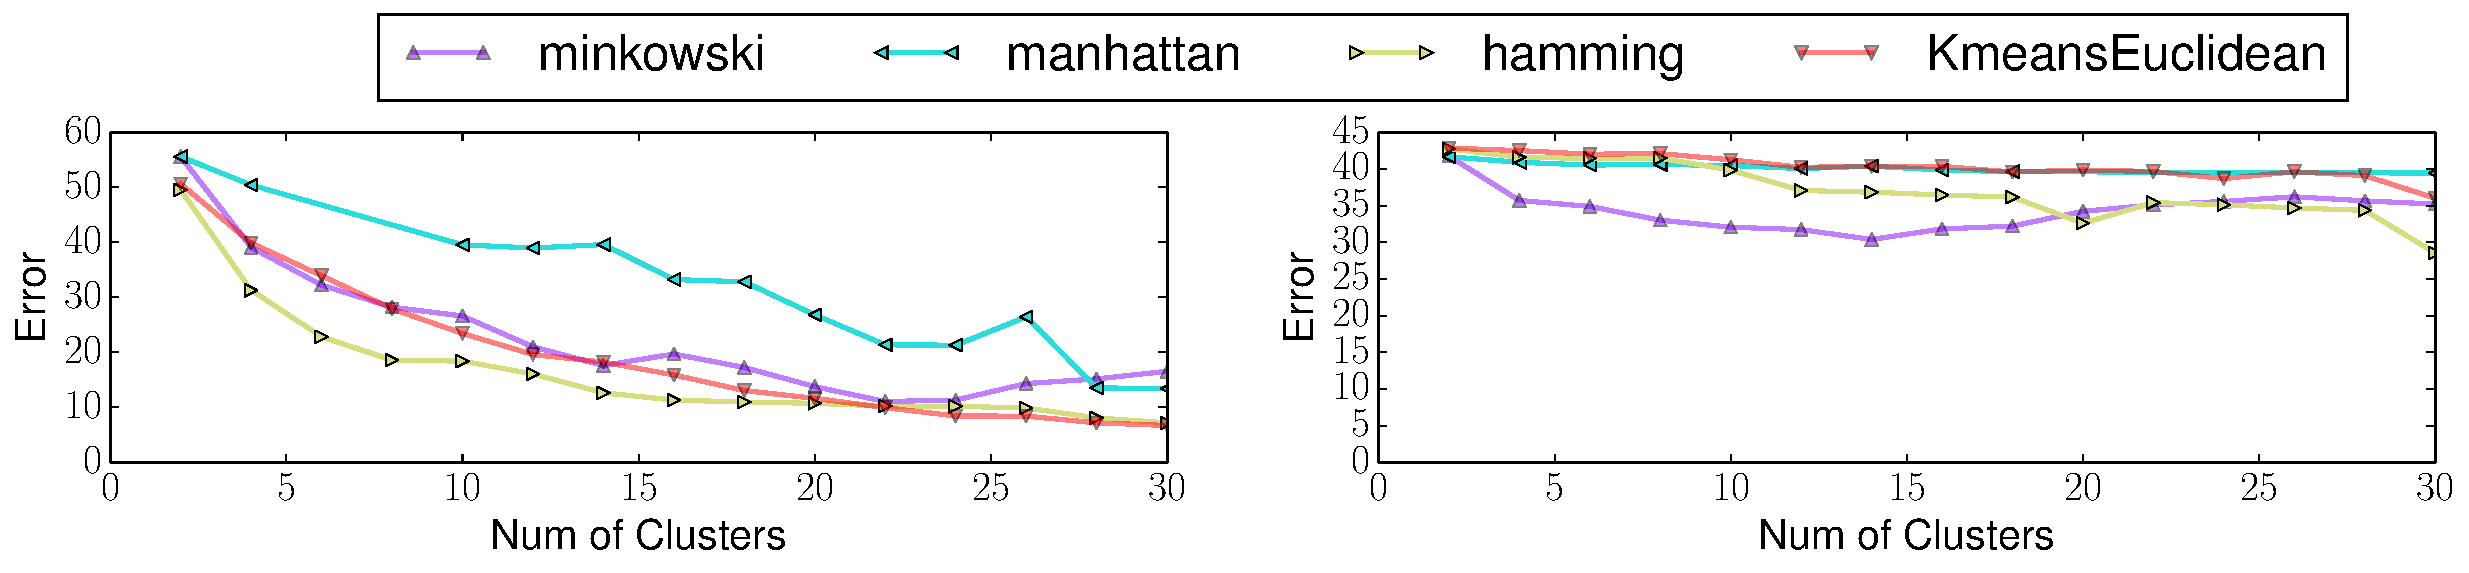
\includegraphics[width=1\textwidth]{QueryLogSummarization/graphics/ErrorVNumCluster.pdf}
 \bfcaption{Error v. Number of Clusters (Left: PocketData, Right: US Bank)}   
 \label{fig:ErrorVNumCluster}
\end{subfigure}
~
%\begin{subfigure}[b]{1\textwidth}
%    \centering      
%    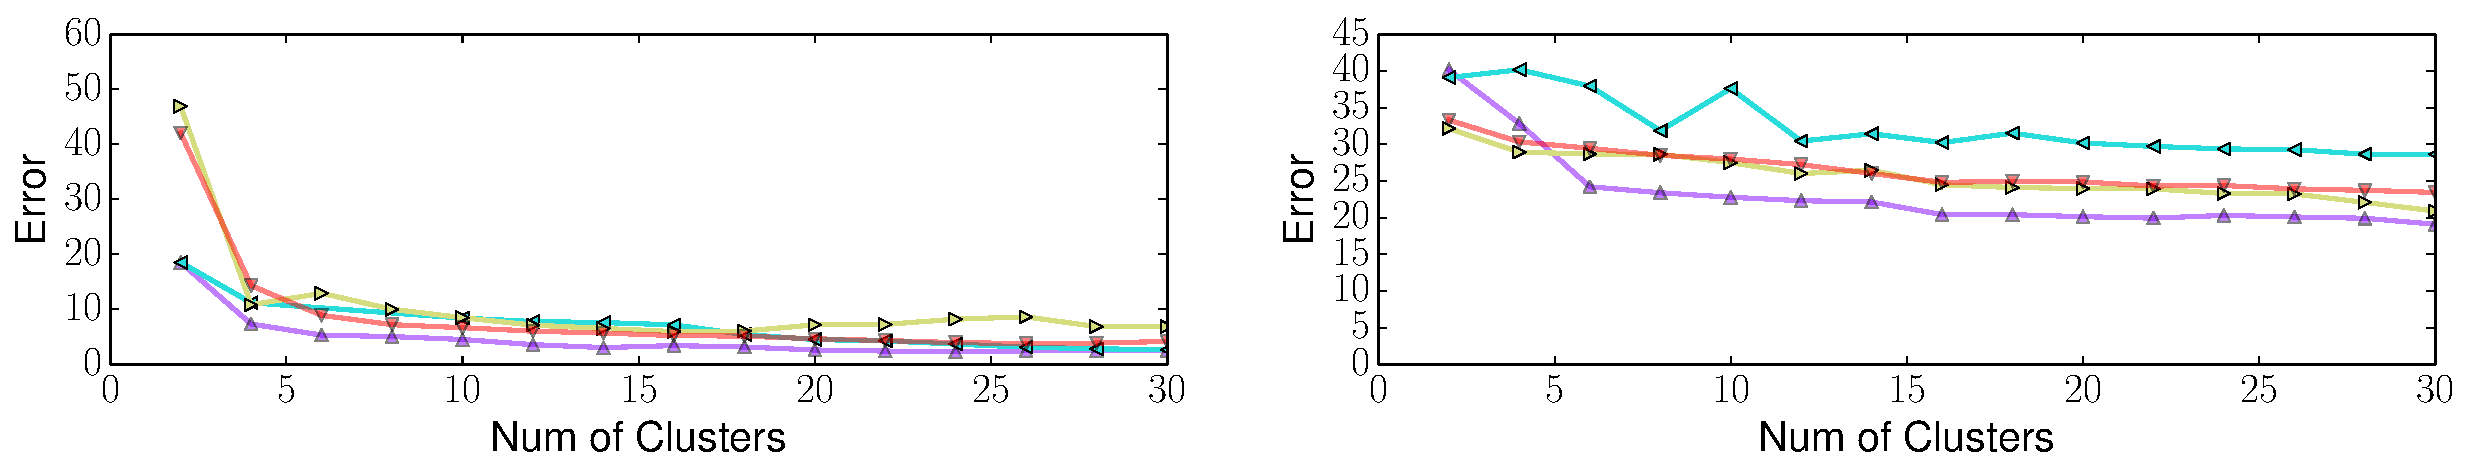
\includegraphics[width=1\textwidth]{QueryLogSummarization/graphics/MultiAdjustedErrorVNumCluster.pdf}
% \bfcaption{Error v. Number of Clusters under multiplicity-aware Clustering (Left: PocketData, Right: US Bank)}   
%\label{fig:MultiAdjustedErrorVNumCluster}
%\end{subfigure}
%~
\begin{subfigure}[b]{0.98\textwidth}
    \centering      
    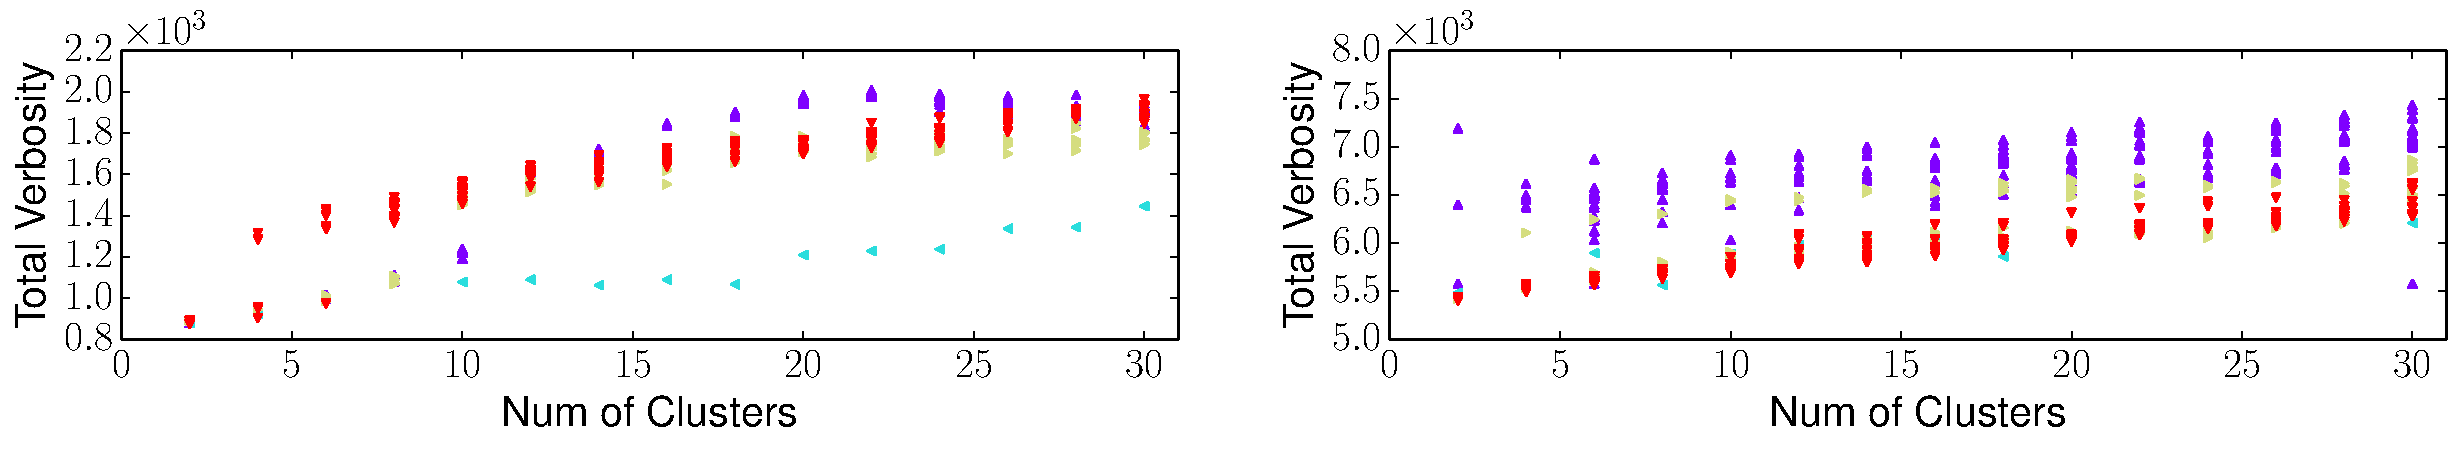
\includegraphics[width=1\textwidth]{QueryLogSummarization/graphics/TotalVerbosityVNumCluster.pdf}
 \bfcaption{Total Verbosity v. Number of Clusters (Left: PocketData, Right: US Bank); 
Each point is the verbosity of one of ten trials.  The Y-axis' lower bound is the verbosity at 1 cluster to better show the change in verbosity.}   
 \label{fig:TotalVerbosityVNumCluster}
\end{subfigure}
~
%\begin{subfigure}[b]{0.98\textwidth}
%    \centering      \includegraphics[width=1\textwidth]{QueryLogSummarization/graphics/ErrorVExpectationOfVerbosity.pdf}
% \bfcaption{Error v. Expectation of Verbosity (Left: PocketData, Right: US Bank)}   \label{fig:ErrorVExpectationOfVerbosity}
%\end{subfigure}
%~
\begin{subfigure}[b]{0.99\textwidth}
    \centering      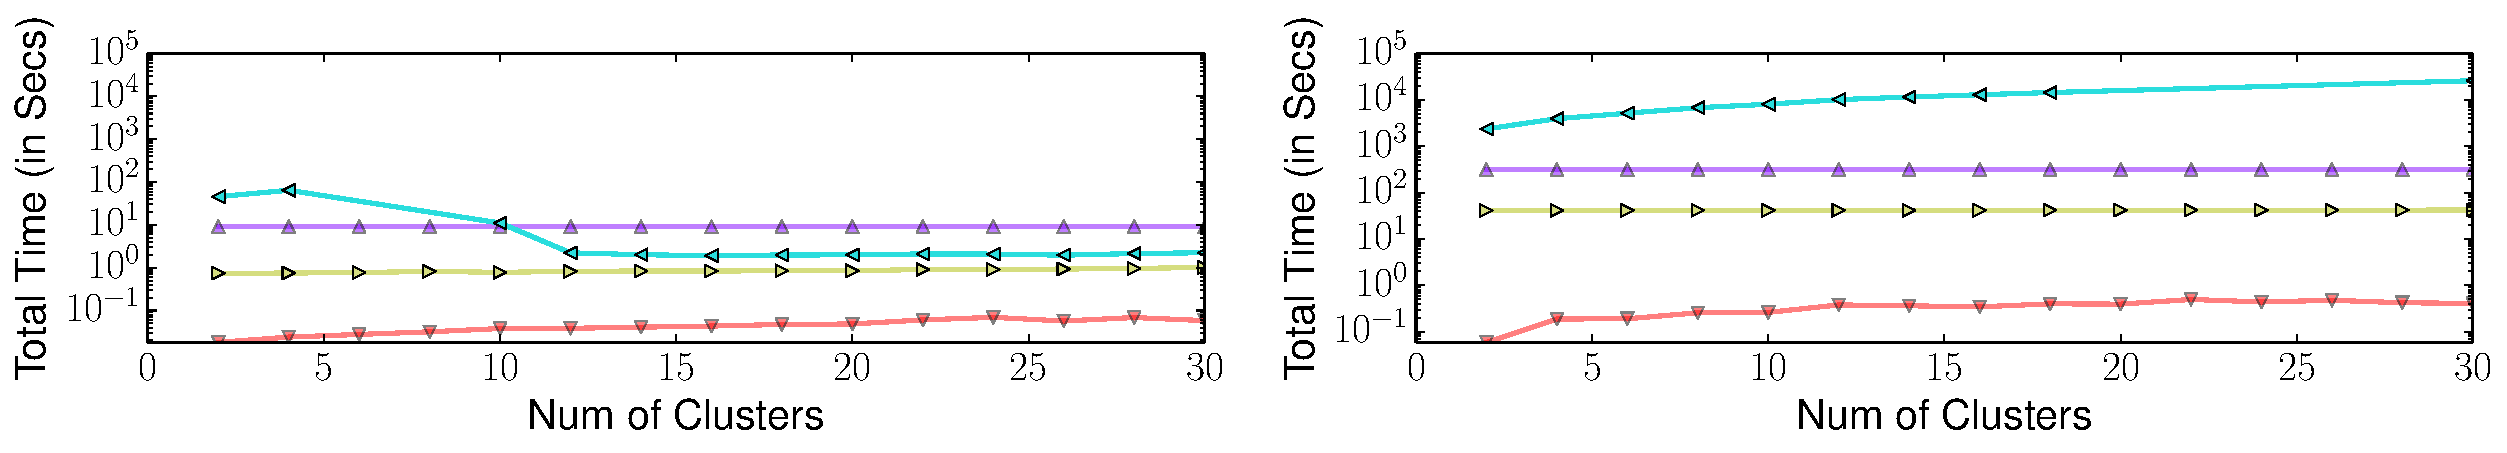
\includegraphics[width=1\textwidth]{QueryLogSummarization/graphics/RunningTimeVNumCluster.pdf}
 \bfcaption{Runtime v. Number of Clusters (Left: PocketData, Right: US Bank)}   \label{fig:RunningTimeVCluster}
\end{subfigure}
~
 \bfcaption{Clustering Schemes Comparison}
 \label{fig:distancemeasurecomparison} 
 \trimfigurewhitespace
\end{figure*}

\section{Pattern Mixture Compression}
\label{sec:constructingencodings}
We are now ready to describe the \systemname compression scheme.
Broadly, \systemname attempts to identify a pattern mixture encoding that optimizes for some target trade-off between Total Verbosity and Error.  
A naive --- though impractical --- approach to finding such an encoding would be to search the entire space of possible pattern mixture encodings.
Instead, \systemname approximates the same outcome by first identifying the naive mixture encoding that is closest to optimal for the desired trade-off.
As we show experimentally, this naive mixture encoding is competitive with more complicated, slower techniques for summarizing query logs.
We also explore a hypothetical second stage, where \systemname refines the naive mixture encoding to further reduce Error.
The outcome of this hypothetical stage has a slightly lower Error and Verbosity, but does not admit efficient computation of database statistics. 

\subsection{Constructing Naive Mixture Encodings}
\label{sec:constructingnaivemixtureencodings}
\systemname searches for a naive mixture encoding that best optimizes for a requested tradeoff between Total Verbosity and Error.  
As a way to make this search efficient, we observe that a log (or log partition) uniquely determines its naive (or naive mixture) encoding. 
Thus the problem of searching for a naive mixture encoding reduces to searching for the corresponding log partitioning.
We further observe that the Error of a naive mixture encoding is proportional to the diversity of the queries in the log being encoded: 
The more uniform the log (or partition), the lower the Error.
Hence, the partitioning problem further reduces to clustering queries in the log by feature overlap.
% \begin{example}
% \label{example:twolevelnaivemixtureencoding}
% Figure~\ref{fig:hierarchicalnaivemixtureencoding} shows an example of constructing a naive mixture encoding from partitioning one cluster into two.
% The naive encodings on the child level (Figure~\ref{fig:childlevel}), each with lower Average Verbosity and Encoding Error, provide a cleaner view of the mixed workload.
% % The Average Verbosity of the resulting naive mixture encoding is lower, as is the generalized Encoding Error.
% However, note that feature \cqword{FROM}{Messages} appears in both children, so the Total Verbosity of the child level is one higher than the parent --- observers see the same feature twice.
% \end{example}
To identify a suitable clustering scheme, we next evaluate four commonly used clustering schemes with respect to their ability to create naive mixture encodings with low Error and Verbosity: (1) KMeans~\cite{DBLP:journals/prl/Jain10} with Euclidean distance (i.e., $l_2$-norm) and Spectral Clustering~\cite{DBLP:journals/jacm/KannanVV04} with (2) Manhattan (i.e., $l_1$-norm), (3) Minkowski (i.e., $l_p$-norm) with $p=4$, and (4) Hamming distances\footnote{We also evaluated Spectral Clustering with Euclidean, Chebyshev and Canberra distances; These did not perform better and we omit them in the interest of conciseness.}.
% \begin{figure}
%  \centering
% \begin{subfigure}{\columnwidth}
%   {\small
%     \begin{tabular}{r|p{60mm}}
%     \textbf{SELECT} & 
%         \texttt{sms\_type},
%         \textcolor{light-gray}{\texttt{external\_ids}},
%         \texttt{\_time},
%         \texttt{\_id}\\ \hline
%     \textbf{FROM} &
%         \texttt{Messages}\\ \hline
%     \textbf{WHERE} &
%         \texttt{(sms\_type=1)} $\wedge$
%         \textcolor{mid-gray}{\texttt{(sms\_type=0)}} $\wedge$
%         \texttt{(status=1)}   
%         $\wedge$~\textcolor{light-gray}{\texttt{(\_time$\geq$14260)}} $\wedge$~\texttt{(transport=3)} 
%     \end{tabular}
%   }
%   \bfcaption{\textit{Parent Level}: Naive encoding of a mixture of two workloads.}
%   \label{fig:parentlevel}
% \end{subfigure}\\[2mm]
% \begin{subfigure}{\columnwidth}
% \hspace*{-1mm}
%   {\small
%     \centering
%     \begin{tabular}{r|p{20mm}}
%     \textbf{SELECT} & 
%         \texttt{sms\_type},\texttt{\_time}
%         \\ \hline
%     \textbf{FROM} &
%         \texttt{Messages}\\ \hline
%     \textbf{WHERE} &
%         \texttt{(sms\_type=1)}$\wedge$ 
%         \textcolor{mid-gray}{\texttt{(sms\_type=0)}}$\wedge$
%         \textcolor{light-gray}{\texttt{(\_time$\geq$14260)}}  
%     \end{tabular}
%     \begin{tabular}{r|p{20mm}}
%     \textbf{SELECT} & 
%         \texttt{\_id}, \textcolor{light-gray}{\texttt{external\_ids}}
%         \\ \hline
%     \textbf{FROM} &
%         \texttt{Messages}\\ \hline
%     \textbf{WHERE} &
%         \texttt{(status=1)}$\wedge$
%         \texttt{(transport=3)} 
%     \end{tabular}
%   }
%   \bfcaption{\textit{Child Level}: Two children encodings that separately summarize each workload.}
%   \label{fig:childlevel}  
% \end{subfigure}\\[2mm]
% \bfcaption{\textbf{Constructing a naive mixture encoding}}
% \label{fig:hierarchicalnaivemixtureencoding}
% \trimfigurewhitespace
% \end{figure}

\tinysection{Experiment Setup}
Spectral and KMeans clustering algorithms are implemented by \textit{sklearn}~\cite{scikit-learn} in Python. 
We gradually increase $K$ (i.e., the number of clusters) for each clustering scheme to mimic the process of continuously sub-clustering the log, tolerating higher Total Verbosity for lower Error.
To reduce randomness in clustering, we run each of them $10$ times for each $K$ and averaging the Error of the resulting encodings.  
We used two datasets: ``US Bank'' and ``PocketData''.  
We describe both datsets and the data preparation process in detail in Section~\ref{sec:commonexperimentsettings}. 
All results for our clustering experiments are shown in Figure~\ref{fig:distancemeasurecomparison}.

\subsubsection{Clustering}
\label{sec:clustering}
We next show that clustering is an effective way to consistently reduce Error, although no one clustering scheme is ideal for all three of Error, Verbosity, and runtime.

\tinysection{More clusters reduces Error}
Figure~\ref{fig:ErrorVNumCluster} compares the relationship between the number of clusters (x-axis) and Error (y-axis), showing the varying rates of convergence to zero Error for each clustering scheme.
We observe that adding more clusters does consistently reduce Error for both data sets, regardless of clustering algorithm or distance measure.
We note that the US Bank dataset is significantly more diverse than the PocketData dataset, with respect to the total number of features (See Table~\ref{table:datasummary}) and that more than $30$ clusters may be required for reaching near-zero Error.
In general, Hamming distance converges faster than other distance measures on PocketData.
Minkowski distance shows faster convergence rate than Hamming within $14$ clusters on the US bank dataset. 
%However, it is also the only one that shows a consistently \textit{increasing} trend in Error when the number of clusters exceeds $22$ for both datasets.
%This is because $l_p$-norm is more aggressive in distinguishing between vectors as $p$ grows (i.e., $l_4$ vs $l_2$) and since the US bank dataset is more diverse, Minkowski helps by separating the highly mixed workloads aggressively.
%But it begins to break down when the data is already well-organized (e.g., being partitioned into more than $22$ clusters).

%\tinysection{Multiplicity-aware Clustering}
%Since the number of feature vectors can be millions or even more, practically we only keep \textit{distinct} feature vectors as the input of clustering schemes.
%We store feature vector frequencies in a separate column called \textit{multiplicities}.
%A multiplicity-ignorant clustering scheme assumes a uniform distribution of queries in the log.
%However, query distributions $p(Q)$ of production database logs are usually skewed.
%For example, routine queries repeat themselves overwhelmingly in the log but contribute to a minority of distinct queries.
%We propose to modify the input of clustering schemes such that distinct feature vectors can be treated \textit{as if they have been replicated}\footnote{Efficiency/Scalability is affected if algorithms are modified.}.
%Specifically, we propose to scale each feature vector by multiplying it with the square root of its multiplicity.
%In the context of KMeans, this is equivalent to the modified objective function: $$\myminl\mysuml_{k=1}^K\mysuml_{i=1}^n m_i||\vec{x}_i-\frac{\vec{c}_k}{\sqrt m_i}||^2$$
%$m_i$ is the multiplicity of row $\vec{x}_i$ and $\vec{c}_k$ is the $k$-th centroid.
%We show the rates of convergence to zero Error for multiplicity-aware clustering schemes in Figure~\ref{fig:MultiAdjustedErrorVNumCluster}.
%By comparing Figure~\ref{fig:MultiAdjustedErrorVNumCluster} with Figure~\ref{fig:ErrorVNumCluster}, we observe that Error of all clustering schemes are significantly reduced and minkowski distance provides the fastest convergence rate of Error.    

\tinysection{Adding more clusters increases Verbosity}
Figure~\ref{fig:TotalVerbosityVNumCluster} compares the relationship between the number of clusters (x-axis) and Verbosity (y-axis).
We observe that Verbosity increases with the number of clusters.
This is because when a partition is split, each feature common to both partitions increases the Verbosity by one.
%as shown in Example~\ref{example:twolevelnaivemixtureencoding}.

\tinysection{Hierarchical Clustering}
The clustering schemes produce non-monotonic cluster assignments. That is, Error can occasionally grow as clusters are added (Figure~\ref{fig:ErrorVNumCluster}). 
An alternative is to use hierarchical clustering~\cite{DBLP:journals/prl/Jain10}, which forces monotonic assignments and offers more dynamic control over the Error/Verbosity tradeoff.

%\tinysection{Error v. Average Verbosity}
%We observe from Figure~\ref{fig:ErrorVExpectationOfVerbosity} that Average Verbosity (x-axis) \textit{positively} correlates with Error (y-axis).
%By comparing Figure~\ref{fig:ErrorVNumCluster} with~\ref{fig:ErrorVExpectationOfVerbosity}, we also observe that the clustering method that achieves lower Error also has lower Average Verbosity.
%Recall that Average Verbosity is the weighted sum of the number of distinct features in each cluster for naive mixture encodings. 
%Misplacing queries with less overlap in features (i.e., less similar) into the same cluster increases its number of distinct features, and Average Verbosity measures the weighted average degree of such misplacement over all clusters. 

\tinysection{Run Time Comparison}
The total runtime (y-axis) in Figure~\ref{fig:RunningTimeVCluster} 
%is measured in seconds and 
includes both distance matrix computation time (if any) and clustering time. 
Note the log-scale: K-Means is orders of magnitude faster than the others.
%with Hamming distance also performing competitively.

%%%%%%%%%%%%%%%%%%%%%%%%%%%%%%%%%%%%%%%%%%%

%\subsubsection{Limitation: Correlated Features}
%\label{sec:limitationsoftraditionaldistancemeasures}
%Most distance measures treat features as if they are independent.
%However, queries that overlap in one feature are likely to overlap in others.
%\begin{example}
%Consider the following example queries, which are similar, but perform different tasks.  
%The first query scans all active conversations where people chat over 30 secs, while the second checks whether active conversations having no chat are blocked. 
%\begin{lstlisting}
%SELECT _id,...,time_stamp
%FROM Conversations WHERE status=active
%AND chat_id NOT NULL AND chat_time>30
%\end{lstlisting} \vspace*{-2mm}
%\begin{lstlisting}
%SELECT _id,...,time_stamp
%FROM Conversations WHERE status=active 
%AND chat_id IS NULL AND blocked=true
%\end{lstlisting}
%\cqword{SELECT}{\_id},\ldots, \cqword{SELECT}{time\_stamp}, \cqword{FROM}{Conversations}, and \cqword{WHERE}{status=active} all appear in both queries.  
%Conversely, there are in total four features uniquely own by each query: \cqword{WHERE}{chat_id NOT NULL}, \cqword{WHERE}{chat_time>30} owned by the former; \cqword{WHERE}{chat_id IS NULL}, \cqword{WHERE}{blocked=true} owned by the latter.
%Mixing these two queries in the same cluster
%Because the number of features shared by both queries dominantly exceeds the most distance measures will treat these queries as being more similar than not.
%However, 
%\end{example}
%Notably, while Hamming distance also suffers from this limitation, it is better than others as a result of considering feature multiplicity (i.e. only exact matches on features contribute to similarity). 

%\subsubsection{Marginal-Aware Distance}
%We account for feature correlations through a new marginal-aware distance (MAD) function (denoted $d_m$).
%For queries $\vec{q}=(x_1,\ldots,x_n)$ and $\vec{q}'=(x_1',\ldots,x_n')$, we define MAD as:
%{\small
%$$d_m(\vec{q},\vec{q}')=p(Q\supseteq\vec{b})\log\left(\frac{p(Q\supseteq\vec{b})}{\min(\;p(Q\supseteq\vec{q}),\; p(Q\supseteq\vec{q}')\;)}\right)$$
%}
%Here, we define $\vec b$ as $(min(x_1,x_1'),\ldots,min(x_n,x_n'))$, or the bag intersection of the two queries.
%Hence, the more likely we are to find the overlapping elements in any query in the log, the higher the distance.
%If the queries themselves are more likely, we would also expect their intersections to be more frequent, so the formula is normalized by the probability of the less likely query.
%MAD is non-negative, symmetric and reaches zero when $\vec{q}$ and $\vec{q}'$ are identical. 

\tinysection{Take-Aways}
%We need multiplicity-aware clustering schemes for workload compression.
For time-sensitive applications, KMeans algorithm is preferred to Spectral Clustering.
With respect to distance measures, minkowski (i.e., $l_p$-norm) with $p=4$ provides the best tradeoff between Error and runtime.

\tinysection{Visualizing Naive Mixture Encoding}
As with normal pattern summaries, naive mixture summaries are also interpretable.
For example a visualization like that of Figure~\ref{fig:screenshots:nocorrelation} can be repeated, once for each cluster.  
For more details, see our accompanying technical report~\cite{DBLP:journals/corr/abs-1809-00405}.

% \subsubsection{Visualizing PocketData}
% To further validate that clustering facilitates efficiently communicating the information content, we offer visualization of PocketData using naive mixture encodings under $8$ clusters in Appendix~\ref{appendix:naivemixtureencodingvisualization}.

\subsection{Approximating Log Statistics}
Recall that our primary goal is estimating statistical properties.
In particular, we are interested in counting the occurrences $\Gamma_\pattern(L)$ (i.e., $p(Q\supseteq\vec b)\cdot |L|$) of some pattern $\pattern$ in the log.
%$$\Gamma_\pattern(L) = |\comprehension{\vec q}{\vec q \in L \wedge \pattern \subseteq \vec q}|$$
Recall that a naive encoding $\naiveencoding$ includes only single-feature patterns (i.e., patterns exactly encoding $p(X_i\ge x_i)$) and that the closed-form representation for the maximum entropy distribution $\overline \rho_{\naiveencoding}$ arises by independence between features (i.e., $\overline \rho_{\naiveencoding}(Q = \vec q) = \prod_{i} p(X_i = x_i)$).
Similarly, we use the independence assumption to estimate:
$$est[\Gamma_\pattern(L)\;|\;\naiveencoding]=\overline \rho_{\naiveencoding}(Q \supseteq \vec b)\cdot |L| = \prod_{i} p(X_i \geq x_i)\cdot |L|$$
%Assuming log distributions allowed by this encoding are equally likely, its maximum entropy distribution $\overline \rho_{\naiveencoding}$ has a closed-form representation.
%Hence, we estimate $\Gamma_\pattern(L)$ through multiplying the probability of the feature occurring by the size of the log: $|L| \cdot \overline \rho_{\naiveencoding}$, or:
%$$est[\;\Gamma_\pattern(L) \;|\; \encoding_L\;] = |L| \cdot \left(\prod_{f \in \encoding\text{ \textbf{where} }f \subseteq \pattern} \encoding[f]\right)$$

This process trivially generalizes to naive pattern mixture encodings by mixing distributions.  
Specifically, given a set of partitions $L_1 \cup \ldots \cup L_K = L$, the estimated counts for $\Gamma_\pattern(L)$ under each individual partition $L_i$ can be computed based on the partition's naive encoding $\naiveencoding_i$, and we then sum up the estimated counts in each partition:
$$est[\;\Gamma_\pattern(L_i)\;|\;\naiveencoding_1, \ldots, \naiveencoding_K\;] = \sum_{i \in [1, K]} est[\;\Gamma_\pattern(L_i)\;|\;\naiveencoding_i\;]$$

\begin{figure*}[h!]
\captionsetup[subfigure]{justification=centering}
    \centering 
    
\begin{subfigure}[b]{0.49\textwidth}
    \centering     
     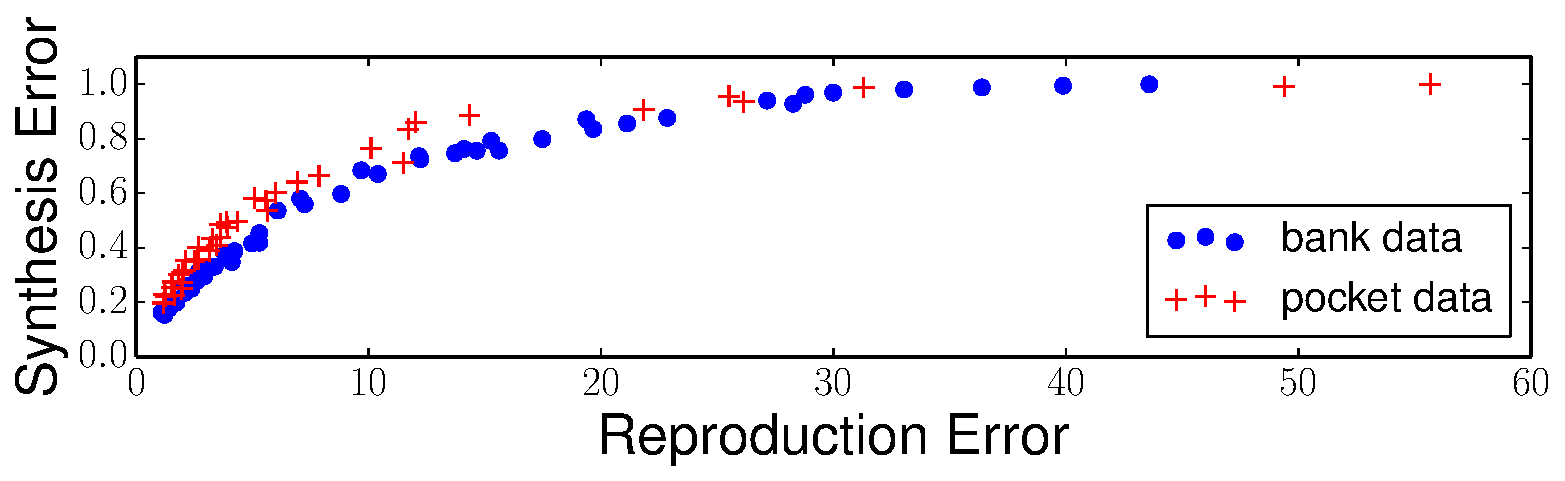
\includegraphics[width=1\textwidth]{QueryLogSummarization/graphics/synthesis_error.pdf}
 \bfcaption{Synthesis Error v. \Errorname}   
 \label{fig:synthesis_error_versus_reproduction_error}
\end{subfigure}
~
\begin{subfigure}[b]{0.49\textwidth}
    \centering      
    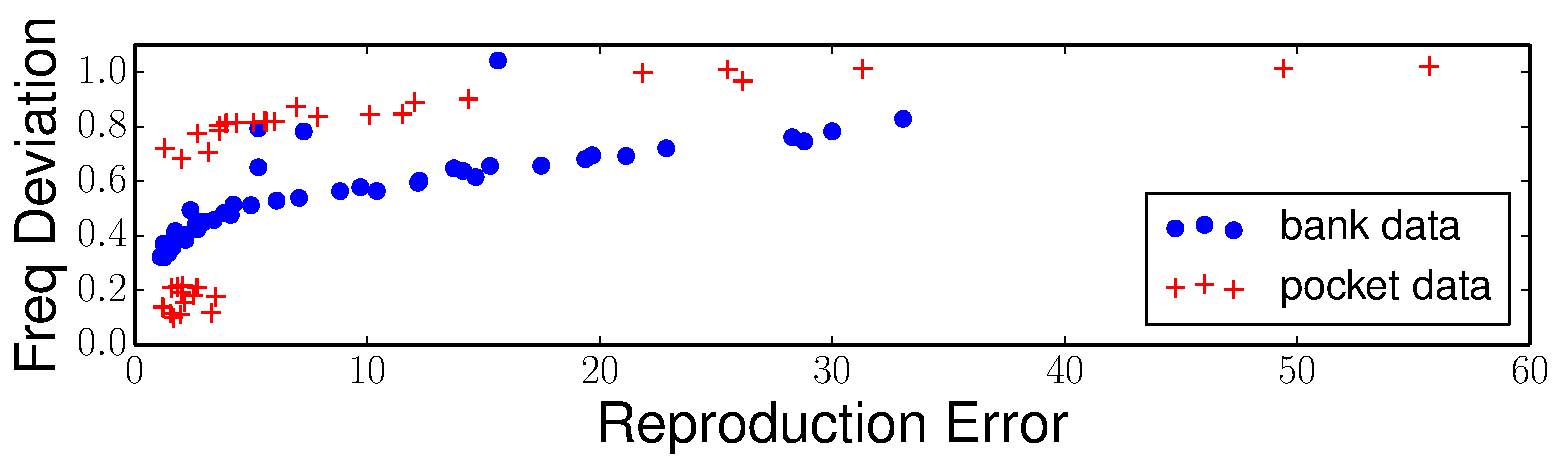
\includegraphics[width=1\textwidth]{QueryLogSummarization/graphics/marginal_deviation.pdf}
 \bfcaption{Frequency Deviation v. \Errorname}   
 \label{fig:marginal_deviation_versus_reproduction_error}
\end{subfigure}

 \bfcaption{Effectiveness of Naive Mixture Encoding}
 \label{fig:effectiveness_of_naive_mixture_encoding} 
 \trimfigurewhitespace
\end{figure*} 

\subsection{Pattern Synthesis \& Frequency Estimate}
In this section, we empirically verify the effectiveness of naive mixture encodings in approximating log statistics from two related perspectives. 
The first perspective focuses on \textit{synthesis error}. 
It measures whether patterns synthesized by the naive mixture encoding actually appear in the log.
From the second perspective, we further investigate the \textit{frequency deviation} of patterns contained in the log.
This evaluates whether a naive mixture encoding computes the correct frequency for patterns of interest to client applications.
Experimental results are shown in Figure~\ref{fig:effectiveness_of_naive_mixture_encoding}.
Both synthesis error and frequency deviation consistently decrease given more clusters.
Furthermore, as we vary the number of clusters, both measures correlate with \errorname.

\noindent \textbf{Synthesis Error}
is measured by $1-\frac{m}{n}$ where $m$ out of $n$ randomly synthesized patterns actually appear in the log.
Intuitively, when synthesis error grows, it is more likely that a pattern from the synthesized log will not appear in the original log (i.e., smaller values are better).
Figure~\ref{fig:synthesis_error_versus_reproduction_error} shows synthesis error (y-axis) versus \errorname (x-axis).
The figure is generated by synthesizing $n=10000$ patterns from each cluster of the log.
Note that different values of $n$ give similar observations.
The overall synthesis error is measured by the average of synthesis errors for all clusters, weighted by the proportion of queries in each cluster.

\noindent \textbf{Frequency Deviation}
is measured for a pattern by $\frac{|est-t|}{t}$ where $t$ stands for true frequency of a pattern and $est$ is the one estimated by the naive mixture encoding.
Since frequency deviation is smaller when evaluated on a pattern contained in the other, as an alternative, we treat each distinct query in the log as a pattern and the frequency deviation on it will be the worst case for all patterns that it contains.
Intuitively, this value captures the percentage error of frequency estimates (i.e., smaller values are better).
For each cluster, we sum frequency deviations on all of its distinct queries and the final frequency deviation for the whole log is an weighted average (same as synthesis error) over all clusters.
Figure~\ref{fig:marginal_deviation_versus_reproduction_error} shows frequency deviation (y-axis) versus \errorname (x-axis).

\subsection{Naive Encoding Refinement}
\label{sec:naivemixtureencodingrefinement}
Naive mixture encodings can already achieve close to near-zero Error (Figure~\ref{fig:ErrorVNumCluster}), have low Total Verbosity, and admit efficiently computable log statistics $\Gamma_\pattern(L)$.
Doing so makes estimating statistics more computationally expensive.
However, as a thought experiment we consider a hypothetical second pass to enrich naive mixture encodings with non-naive patterns.
We start by considering the simpler problem of identifying the \emph{individual} non-naive pattern that maximally reduces the \errorname of a naive encoding.

\tinysection{Feature-Correlation Refinement}
Recall that under naive encodings, we have a closed-form estimation $\overline \rho_{\naiveencoding}(Q \supseteq \vec b)$ of pattern frequencies $p(Q\supseteq\vec b)$.
We thus define the \textit{feature-correlation} of pattern $\vec b$ as the log-difference from its actual frequency to the estimate.
$$fc(\vec b, \naiveencoding) = |\log\left(
    p(Q \supseteq \vec b)
\right) - \log\left(
  %\prod_{i} p(X_i \geq x_i)
  \overline \rho_{\naiveencoding}(Q \supseteq \vec b)
\right)|$$
Intuitively, patterns with higher feature correlations carry more information content of the log that its naive encoding ignores, making them ideal candidates for addition to the naive encoding.
For two patterns with the same feature-correlation, the one that occurs more frequently~\cite{DBLP:journals/datamine/HanCXY07} will have greater impact on \errorname. 
As a result, we compute an overall score for ranking individual patterns:  
$$corr\_rank(\vec{b})=p(Q \supseteq \vec b) \cdot fc(\vec b, \naiveencoding)$$
We show in Section~\ref{sec:motivateencodingerror} that $corr\_rank$ closely correlates with \errorname.
That is, a higher $corr\_rank$ value indicates that a pattern produces a greater reduction in \errorname if introduced into the naive encoding.

\tinysection{Pattern Diversification}
In general, we would like to identify a \emph{set} of patterns.
The greedy approach that adds patterns one by one based on their ranking scores $corr\_rank$ is unreliable, as modifying the naive encoding invalidates the closed-form estimation $\overline \rho_{\naiveencoding}(Q \supseteq \vec b)$ that score $corr\_rank$ relies on.
In other words, we can not sum up $corr\_rank$ scores of patterns in a set to rank its overall contribution to \errorname reduction, as information content carried by patterns may overlap.
To counter such overlap, or equivalently to \textit{diversify} patterns, a search through the space of pattern-sets is needed.
This type of diversification is commonly used in pattern mining applications, but can quickly become expensive.
As we show experimentally in Section~\ref{sec:motivatepatternmixturesummaries}, the benefit of diversification is minimal.
%\subsection{Error Bound Analysis}
%\begin{proposition}
%\label{pigeonhole}
%Given Bernoulli distributions 
%$$X_i \sim \operatorname{\mathit{Bernoulli(p_i)}}, i=1\ldots n, n\geq 2$$
% Without loss of generality, suppose $\forall i,p_i\geq 0.5$\footnote{if $p_i<0.5$ replace variable $X_i$ with $X'_i$ where $X'_i=0 \equiv X_i=1$}, the joint probability 
% $$p(X_1=1,\ldots,X_n=1)\in \left[\mysuml_{i=1\ldots n}p_i-n+1,\myminl_{i=1\ldots n}(p_i)\right]$$
%\end{proposition}
%\begin{proof}
%Start from the case $i=2$ where $p_1,p_2$ are both fixed and greater than equals $0.5$. To obtain the lower bound of $p(X_1=1,X_1=2)$, we make best-effort to rearrange the assignments of $X_1=1$ on instances of $(X_1,X_2)$, such that $X_1=1$ never co-occurs with $X_2=1$ in the same instance. However, according to pigeon hole principle, under the constraints that $X_1=1$ and $X_2=1$ must occupy $p_1,p_2$ proportion of all instances respectively, there is at least $p_1+p_2-1$ proportion where $X_1=1$ and $X_2=1$ co-occur. In other features, $p(X_1=1,X_2=1)\geq p_1+p_2-1$. For the upper bound, $p(X_1=1,X_2=1)$ can neither exceed $p(X_1=1)$ nor $p(X_2=1))$. Hence $p(X_1=1,X_2=1)\in [p_1+p_2-1,\min(p_1,p_2)]$. Using mathematical reduction, suppose $i=k$, $p(X_1=1,\ldots,X_k=1)\in [\mysuml_{i=1\ldots k}p_i-k+1,\myminl_{i=1\ldots k}(p_i)]$. When $i=k+1$, we create a variable $X$ where $(X_1=1,\ldots,X_k=1) \equiv X=1$. In other features, $p(X_1=1,\ldots,X_{k+1}=1)\equiv p(X=1,X_{k+1}=1)$. Similar to the case when $i=2$, $p(X=1,X_{k+1}=1)\geq p(X=1)+p(X_{k+1}=1)-1 \geq \mysuml_{i=1\ldots k}p_i-k+1+p_{k+1}-1=\mysuml_{i=1\ldots k+1}p_i-(k+1)+1$. Also $p(X=1,X_{k+1}=1)\leq \min(p(X=1),p(X_{k+1}=1))\leq \min(\myminl_{i=1\ldots k}(p_i),p_{k+1}) =\myminl_{i=1\ldots k+1}(p_i)$.
%\end{proof}
%Proposition~\ref{pigeonhole} reveals that the $\log$ difference between the joint probability $p(X_1=1,\ldots,X_n=1)$ and its possible estimations (e.g.$\myPil_{i=1\ldots n}p(X_i=1)$) is bounded by $\log\frac{\myminl_{i=1\ldots n}(p_i)}{\mysuml_{i=1\ldots n}p_i-n+1}$. With increased $p_i,i=1\ldots n$, this bound get squeezed.

%In fact, for case $i=2$, the bounds for all 4 assignment cases of $(X_1,X_2)$ can be similarly obtained by pigeon hole principle:
%\begin{enumerate}
%\item $p(X_1=0,X_2=0)\in [0, \,min(1-p_1,1-p_2)]$; 
%\item $p(X_1=1,X_2=1)\in [p_1+p_2-1,\,min(p_1,p_2)]$;
%\item $p(X_1=0,X_2=1)\in [\max(0,p_2-p_1),\,\min(1-p_1,p_2)]$;
%\item $p(X_1=1,X_2=0)\in [\max(0,p_1-p_2),\,\min(1-p_2,p_1)]$.
%\end{enumerate}
%We come to the conclusion that increasing $p_1$ and $p_2$ squeezes bounds for all cases simultaneously. Using mathematical reduction similar in proposition~\ref{pigeonhole}, the conclusion for case $i=2$ can be generalized to cases where $i=n$. 

%In practice, the target vectors $(\ldots,x_i,\dots)$ for clustering can be viewed as multivariate observations of variables $(\ldots,X_i,\ldots)$ where $X_i$ can take multiple values $\sup X_i>1$. Suppose $Y_{i,k}=1\equiv X_i\geq k$, almost all traditional distance metrics tend to consistently increase either $p(Y_{i,k}=1)$ or $p(Y_{i,k}=0)$ for all variables $Y_{i,k}$ within each cluster. Thus the error of approximating the joint distribution $(Y_{1,1},\ldots,Y_{1,\sup X_1},\ldots,Y_{n,\sup X_n})$ within each cluster assuming independence among $Y_{i,k}$ consistently reduces. 



